\section{non-hydrostatic finite volume Chombo AMR model on the cubed sphere}
Discuss hydrostatic vs non-hydrostatic

\section{Governing Equations}

The flux form of the shallow water equations is:
\begin{equation}
	\frac{\partial h\mathbf{u}}{\partial t}+\nabla\cdot(\mathbf{u}h\mathbf{u})=-f\mathbf{\hat{k}}\times h\mathbf{u}-Gh\nabla H
\end{equation}
\begin{equation}
	\frac{\partial h}{\partial t}+\nabla\cdot(h\mathbf{u})=0
\end{equation}
where $H=h+z_{s}$ with $h$ the fluid height and $z_{s}$ the height of the underlying topography. $\mathbf{u}$ is the velocity vector, and $\mathbf{\hat{k}}$ is the unit vector perpendicular to the surface.  The Coriolis parameter is $f$ while $G$ is the gravitational acceleration constant. In equiangular coordinates, the shallow water equations on a cubed sphere can be written as:
\begin{equation}
     \label{eq:SWcubesphere}
     \frac{\partial}{\partial t}\left(J\mathbf{U}\right) + \nabla\cdot(J\mathbf{\vec{F}}) = J\mathbf{\Psi}
\end{equation}
where
\begin{equation}
      \mathbf{U}= \left( \begin{array}{c}
       h \\
       h u^\alpha \\
       h u^\beta
       \end{array} \right), \
       \mathbf{F}^k = \left( \begin{array}{c}
        h u^k \\
        hu^{k}u^{\alpha}+g^{k \alpha}\frac{1}{2}Gh^{2} \\
        hu^{k}u^{\beta}+g^{k \beta}\frac{1}{2}Gh^{2} 
        \end{array} \right), \
        \mathbf{\Psi} =  \left( \begin{array}{c}
        0 \\
        \mathbf{\Psi}_{M}^{\alpha}+\mathbf{\Psi}_{C}^{\alpha}+\mathbf{\Psi}_{B}^{\alpha} \\
        \mathbf{\Psi}_{M}^{\beta}+\mathbf{\Psi}_{C}^{\beta}+\mathbf{\Psi}_{B}^{\beta} \\
         \end{array} \right).
\end{equation}
Here $\mathbf{U}$ contains the conserved variables while the first term in $\mathbf{F}^{k}$ is the "mass" flux vector and the bottom two terms are the "momentum" flux tensors.  $J$ is the Jacobian on the manifold and $g^{nk}$ is the contravariant cubed sphere metric with $k$ and $n$ $=\{\alpha,\beta\}$.  The $\mathbf{\Psi}_{M}$, $\mathbf{\Psi}_{C}$, and $\mathbf{\Psi}_{B}$ terms represent the metric, Coriolis, and bottom topography source terms respectively (See \cite{McCorquodale:2014rw} for the full representations of the source terms). 

In three dimensions very similar.

\section{The cubed-sphere grid}
The cubed-sphere grid was developed by \cite{Sardony} as a solution to the "pole problem" that traditional spherical latitude-longitude grids 
possess. In the latitude-longitude  projection, converging meridians create singularities at North and South poles with computationally inefficient 
small grid spacing near the poles. The cubed-sphere grid avoids this "pole-problem" by projecting a gridded cube onto the surface of a sphere. The grid replaces the two strong singulars of poles with eight weaker singularities at
the corner points of the originally cube.  The cubed-sphere grid also provides a near uniform tiling of the sphere compared with the
large changes in grid spacing on the latitude-longitude mesh. However, the grid design
was not competitive with existing models as the overhead cost of storing the grid structure computationally
were too significant. The use of the cubed-sphere was revived in the mid 1990s in a shallow water 
model by \cite{Ronchietal}. Since then the cubed-sphere grid has been implement in several shallow water models and 
a few full atmospheric
models including the hydrostatic Community Atmosphere Spectral Element Model (CAM-SE) \citep{dennis2012cam}, the
non-hydrostatic Tempest model \citep{ullrich2014global,guerra2016high}, and the
Geophysical Fluid Dynamics Laborator's Finite-Volume Cubed-Sphere Dynamical Core (FV3) \citep{lin2004vertically,Harris:2013n}.
In 2016, the National Weather Service selected the cubed-sphere FV3 dynamical core to be implemented in the new version
of the Global Forecast System, its main weather forecast model, which will be operational in 2019.
This growth in use of the cubed sphere grids is a result of the develop of massively
parallel computing systems on which GCMs can now be ran. 
The regular grid structure on each panel allows the computational grid to be efficiently distributed
across these large parallel systems. This regularity also allows additional grid cells to be added or 
removed for variable resolution with more ease compared to unstructured geodesic (icosahedral) grids or the 
more complex Yin-Yang grid.

\begin{figure}[htp]
\centerline{
\includegraphics[width=4in]{ModelDescription/cubedsphere12456.pdf} % was cubedsphere2dreal                                                                                        
}
\caption{
A cubed-sphere grid, shown with labels on panels.
% The surface of the unit sphere in real space.                                                                                                              
Panels 1 -- 4 all straddle the equator
($z = 0$) of the unit sphere.
Panel 5 is centered on the north pole ($z = +1$),
panel 6 on the south pole ($z = -1$).
On the cubed-sphere grid shown here,
$N_{\rm c} = 16$ (each panel contains $16 \times 16$ grid cells).
}
\label{fig:cubedsphere2dmaps}
\end{figure}

The cubed-sphere grid consists of cubed with six Cartesian panels inflated out to form a spherical shell. 
There are multiple ways to map the grids of each panel to the sphere (see \cite{Putnam:2007cs} for a review
of several cubed sphere grids).  The Chombo-AMR model uses gnomonic equiangular cubed-sphere grid, where the
gridlines on each panel have equally spaced central angles relative to the center of the sphere. This projection
gives a quasi-uniform spherical grid. The gird does not have perfectly uniform grid sizes, but as resolution increases
the ratio between the largest and smallest grid cells converges to $\sqrt{2}$, the smallest ratio of cubed-sphere
grids. Figure \ref{fig:cubedsphere2dmaps} depicts the equiangular cubed-sphere grid.

The equiangular coordinates for the cubed-sphere grid are given as $(\alpha, \beta, n_p)$, 
with central anngles $\alpha, \beta \in [-\frac{\pi}{4},\frac{\pi}{4}]$ and the panel number $n_p \in [1,2,\dots, 6]$. 
By convention, panels 1-4 are along the equator and panels 5 and 6 are centered on the north and south poles
respectively as seen Fig. \ref{fig:cubedsphere2dmaps}. The discrete resolution of the cubed-sphere grid is represented as  $c\{N_c\}$ where $N_c$
denotes the number of grid cells in each direction on the six panels.  A
list of properties of the equiangular cubed-sphere grid, including the
approximate grid spacings, and comparable resolutions for other coordinate systems, is given in
Table~\ref{tb:grids} for several resolutions.

\begin{table}[t]
    \caption{Properties for several cubed-sphere grid resolutions where 
    $N_c$ is the number of cells along an edge of a cubed-sphere panel.
    Here the number of cells is the total number of grid cells 
    ($N_c^2 \times 6$), $\Delta x$ is the approximate grid spacing, 
    $A_{avg}$ is the average area of a grid cell, $A_{min}/A_{max}$ is the
    ratio between the minimum and maximum cell areas, Eq.  Res.  is the
    grid resolution in degrees given by $90^\circ / N_c$, and $RLL_{equiv}$
    is the equivalent grid spacing on a regular latitude-longitude
    grid with the same total number of cells.}%
    \label{tb:grids}
    \begin{center}
    \begin{tabular}{cccrccc}
            \hline
            Resolution ($N_c$) & No. of cells       & $\Delta x$ (km) & $A_{avg} (\mbox{ km}^2)$ & $A_{min}/A_{max}$ & Eq. Res.     & $RLL_{equiv}$ \\ 
            \hline
            \hline
            c$32$              & $6.14 \times 10^3$ & $313$           & $8.302 \times 10^{4}$    & $0.7249$          & $2.81^\circ$ & $3.25^\circ$  \\ 
            c$64$              & $2.46 \times 10^4$ & $156$           & $2.076 \times 10^{4}$    & $0.7159$          & $1.41^\circ$ & $1.62^\circ$  \\ 
            c$128$             & $9.83 \times 10^4$ & $78.2$          & $5.189 \times 10^{3}$    & $0.7115$          & $0.70^\circ$ & $0.82^\circ$  \\ 
            c$256$             & $3.93 \times 10^5$ & $39.1$          & $1.297 \times 10^{3}$    & $0.7093$          & $0.35^\circ$ & $0.41^\circ$  \\ 
            c$512$             & $1.57 \times 10^6$ & $19.5$          & $3.243 \times 10^{2}$    & $0.7082$          & $0.18^\circ$ & $0.20^\circ$  \\ 
            c$1024$           & $6.29 \times 10^6$ & $9.77$          & $8.107 \times 10^{1}$    & $0.7076$          & $0.09^\circ$ & $0.10^\circ$  \\ 
            c$2048$           & $2.52 \times 10^7$ & $4.89$          & $2.027 \times 10^{1}$   & $0.7074$          & $0.04^\circ$ & $0.05^\circ$ \\
            \hline
        \end{tabular}
    \end{center}
\end{table}

%%%%%%%%%%%%%%%%%%%%%%%%%%
\section{Finite Volume Discretization}
Finite-volume methods were first developed in 
other areas of hydrodynamics such as astrophysics 
and aerospace for modeling high speed flows and shockwaves and 
trace their origins back to the conservative finite-volume methods developed
by \cite{Godunov}. These methods were extend to second order by the work of Bram
van Leer in \cite{van Leer}
and later \cite{Collela} developed the piecewise-parabolic method (PPM), a third-order
Godunov-type finite volume method.
Early adaptations of finite-volume methods for atmospheric advection problems
by \cite {rood 1987}, \cite{Carpenter et al. (1990)}, and \cite{Allen1991} led to the development 
a finite-volume dynamical core for the shallow water equations \citep{Lin Rood} and later the full 3D
equations of motion \citep{Lin2004}
Use of finite-volume methods in GCMs has grown, especially with the development of variable resolution. Recently developed models that utlize a finite volume dynamical core include GFDL's FV3, NCAR's Model for Prediction Across Scales (MPAS), and Max-Planck-Institut's ICOsahedral Non-hydrostatic model.
A key advantage of finite volume methods is that they are conservative so they can preserve properties like mass and maintain high accuracy. Additionally, finite-volume methods can be easily formulated for moving or adaptive meshes.

  The finite volume dynamical core uses a volume integral formulation of the equations of motions. 
       In the finite volume approach to discretizing the non-hydrostatic equations, we integrate the equations of motions over the 
       volume of a grid cell
       The Chombo-AMR model uses a conservative 4th order finite-volume scheme to solve the shallow water equations.  Applying a method-of-lines approach, we integrate the SWEs (Equation \ref{eq:SWcubesphere}) over grid cell $V_{i,j}$, make use of Gauss' divergence theorem, and represent the integrals in terms of averages over $V_{i,j}$ and its faces to obtain the discretized volume averaged formulation: 
       \begin{align}
       \frac{d}{dt} \langle J \mathbf{U} \rangle_{i,j}
       = & - \frac{1}{\Delta \alpha} 
       \left( \langle J \mathbf{F}^\alpha \rangle_{i + \frac{1}{2},j} -
       \langle J \mathbf{F}^\alpha \rangle_{i - \frac{1}{2},j} \right)
      - \frac{1}{\Delta \beta}
      \left( \langle J \mathbf{F}^\beta \rangle_{i,j + \frac{1}{2}} -
      \langle J \mathbf{F}^\beta \rangle_{i,j - \frac{1}{2}} \right)
      + \langle J \mathbf{\Psi} \rangle_{i,j} .
      \label{eqn:PDEAveraged}
      \end{align}
 where $\Delta\alpha=\Delta\beta=\frac{\pi}{2N_c}$ are the grid spacing on the equiangular grid, $\langle A \rangle_{i,j}$ represents the average of a quantity $A$ over $V_{i,j}$, and $\langle A \rangle_{i \pm \frac{1}{2},j \pm \frac{1}{2}}$ denote the averages over the faces of $V_{i,j}$,.

   The fluxes at the faces of each grid cell are then obtained via a complex centered spatial interpolation involving deconvolving, interpolating and then convolving the cell values to maintain 4th order accuracy (see \cite{McCorquodale:2014rw} for a full description).  Ghost cells are created by interpolating from stencils of nearby cells (Figure \ref{fig:ghostcellstens}) at boundaries between panels and between block-structures of different resolutions.  
   \begin{figure}[h]
   \centerline{ 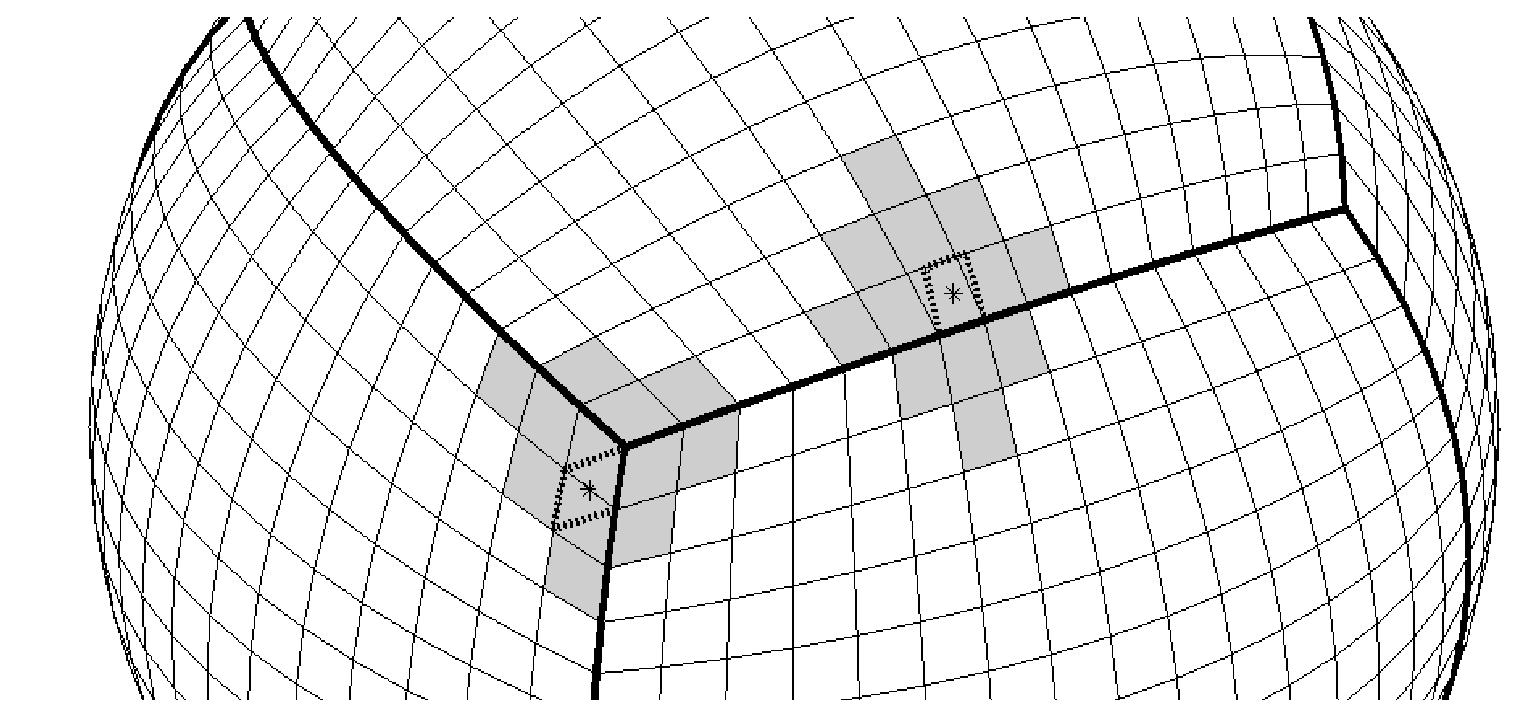
\includegraphics[width=.7\textwidth]{ModelDescription/CSstencilUniform} }
   \caption{Sample interpolation stencils (shaded cells) of two different ghost cells marked with a * at the boundaries of a panel.}
   \label{fig:ghostcellstens}
   \end{figure}
   
   A classical fourth-order explicit Runge-Kutta method is used to advance Equation \ref{eqn:PDEAveraged} in time, which can be written in the form
   \begin{align}
      \frac{d}{dt} \langle J \mathbf{U} \rangle_{i,j}
       = K ( \langle J \mathbf{U} \rangle )_{i,j}
       \label{eqn:PDEAveragedK}
   \end{align}
   such that $K\left(\langle J\mathbf{U} \rangle\right)_{i,j}$ equals the right hand side of Equation \ref{eqn:PDEAveraged}.  Integrating Equation \ref{eqn:PDEAveragedK} over time step $\Delta t$  using the classical Runge-Kutta method with $\langle J \mathbf{U} \rangle^{(0)}$ as the initial value gives the following equations:
   \begin{align}
      & & k_1 & = K(\langle J \mathbf{U} \rangle^{(0)} ) \Delta t; \label{eqn:k1} \\
      \langle J \mathbf{U} \rangle^{(1)} & = \langle J \mathbf{U} \rangle^{(0)} + \frac{k_1}{2} ; &
      k_2 & =   K(\langle J \mathbf{U} \rangle^{(1)} ) \Delta t; \label{eqn:k2} \\ 
      \langle J \mathbf{U} \rangle^{(2)} & = \langle J \mathbf{U} \rangle^{(0)} + \frac{k_2}{2} ; &
      k_3 & =  K(\langle J \mathbf{U} \rangle^{(2)} ) \Delta t; \label{eqn:k3} \\
      \langle J \mathbf{U} \rangle^{(3)} & = \langle J \mathbf{U} \rangle^{(0)} + k_3 ; &
       k_4 & = K(\langle J \mathbf{U} \rangle^{(3)} ) \Delta t \label{eqn:k4} 
    \end{align}
    so that the solution at $t+\Delta t$ is
    \begin{equation}
        \langle J \mathbf{U} \rangle(t^n + \Delta t) = 
        \langle J \mathbf{U} \rangle(t^n) + \frac{1}{6} (k_1 + 2 k_2 + 2 k_3 + k_4) +
        O((\Delta t)^5).
    \end{equation}
    
%%%%%%%%%%%%%%%%%%%
\section{Chombo AMR framework}
The adaptive mesh refinement (AMR) is based on the Chombo library for parallel AMR.   The Chombo library provides a set of tools for finite-difference and finite-volume methods for solving partial differential equations on block-structured AMR grids \citep{colella2000chombo}.  It is a highly-scalable solver that has been shown to scale to $\mathcal{O}(10^{5})$  processors for hyperbolic and elliptical equations related to gas dynamics.    The AMR structure allows refinement around an unlimited number of targeted features and at various levels of refinement. 
   
    AMR calculations are performed on a hierarchy of nested-mesh levels, with a predefined refinement ratio (e.g. 2, 4, or 8) between adjacent levels.  An intermediate level must have enough cells separating the finer and coarser levels to allow interpolation of ghost cells for the finer level.  Levels are grouped into sections of grid cells, called "boxes", in order to perform calculations on large parallel platforms efficiently.  Figure \ref{fig:test1} shows a sample layout of refinement levels and boxes.  AMR grid levels are advanced in time through a sub-cycling process.  The process is outlined in Figure \ref{fig:timesubcycle} (see \cite{McCorquodale:2014rw} again for full details).
        \begin{figure}[h]
 		\centering
  		\includegraphics[width=.6\linewidth]{ModelDescription/amr_block_example}
  		\caption{From \cite{GuzikETAL:2013}, this figure shows a three level grid hierarchy with a x2 refinement ratio between levels.  The block structure is depicted by bolded lines.  Note that the finest layer is nested within the middle layer to allow for the interpolation of ghost cells.  Ghost cells for the middle layer are shown by dashed lines.}
  		\label{fig:test1}
	\end{figure}
	
	\begin{figure}[h]
 		\centering
  		\includegraphics[width=.8\linewidth]{ModelDescription/Time_subcycle_chart}
  		\caption{This diagram depicts the time advancement processes for AMR. The $l$ level is advanced first.  Ghost cells for the $l+1$ level are interpolated both at time $t$ and then from intermediate time steps. The $l+1$ level is then advanced, forward in time; and once a sub-cycle is complete, averages and fluxes are updated back to the coarser level.  This process is cascaded down to the highest refinement level.  The order in which levels are advanced through the sub-cycling is shown by the black arrows.}
 		 \label{fig:timesubcycle}
	\end{figure}
    
    New levels are added whenever the refinement criteria are reached at the current level.  The mesh can be refined up to a predefined number of levels.   AMR-Chombo has a range of possible refinement criteria.  Currently it can base refinement on the gradient or absolute value of vorticity, height, a tracer field, and topography.    The criteria can be set to increase with refinement level or remain constant.  For example, the c256 level would have to observe a higher vorticity than the c64 level to refine further.  Furthermore, new refinement criteria can easily be created and implemented. 
    
%%%%%%%%%%%%%%%%%%%
\section{Shallow Water model setup}


Because the shallow-water equations mimic atmospheric flow in a single layer, 
they serve as a common test bed for atmospheric model development. The shallow-
water equations describe the behavior of a homogenous, incompressible, 
and inviscid fluid in a shallow layer. While sound waves are not supported, the shallow-
water equations are able to resolve Kelvin, Inertia-Gravity, and non-linear 
Rossby waves. By capturing these key wave 
propagations mechanisms, the shallow-water equations retain some of the
most pertinent dynamical features found in the real atmosphere and in 
full three dimensional atmospheric GCMs while staying relatively simple enough to enable 
detailed investigations of a model's dynamical components. A shallow-water model provides
a basic test of horizontal and temporal discretization schemes to determine which numerical
schemes are effective for atmospheric flows without requiring the effort of building a complete
complex model. With the extensive use shallow water models, a wide range test cases have
been developed for the shallow-water equations to evaluate various characteristics of the numerical
schemes. Test cases serve as a useful comparison benchmarks with existing models to 
determine the effectiveness of new numerical technics.
Many test cases consists of simple artificial 
flows with analytical solutions while others have more complex realistic flows without 
an analytic solution and use high resolution runs from existing models as a comparison.
Common test cases implemented in today's literature included
the now canonical test case suite of \cite{Williamson:1992kx} as well as more recently
developed tests including the barotropic instability of \cite{Galewsky:2004uq}. In
our assessment of the AMR model, we implement several established test cases and also
develop several new ones.


\section{3D Model setup}
